\section{Terraform e OpenStack}

\subsection{Introduzione}
Durante lo svolgimento di questo progetto io e il mio collega Sauro abbiamo deciso di prendere due direzioni diverse per quanto riguarda lo studio dell'integrazione tra Terraform e OpenStack: io ho approcciato il provisioning delle risorse tramite Terraform dal punto di vista di un utente che utilizza OpenStack come cloud provider per ospitare le proprie applicazioni, mentre il mio collega si è concentrato maggiormente sul provisioning delle risorse dal punto di vista dell'amministratore del cloud.

L'approccio che ho utilizzato per questo studio è stato iterativo: ho iniziato con un progetto molto semplice che consisteva nel creare una sola istanza per poi arrivare alla terza iterazione ad un progetto molto più complesso che utilizza tutte le possibili risorse offerte dal nostro cloud OpenStack e simula in maniera abbastanza realistica quello che potrebbe essere un caso d'uso reale. Nelle sezioni seguenti saranno descritti nel dettaglio tutti i progetti Terraform che ho realizzato.

\subsection{Progetto 1: istanza}

Come accennato in precedenza il primo progetto consiste solamente nel deployment di un'istanza tramite Terraform. L'unico file presente è \verb|main.tf| che al suo interno contiene 3 blocchi che verranno riportati e descritti di seguito.

\paragraph{Blocco terraform.}
Il primo blocco è di tipo \code{terraform}, ovvero quello che contiene le impostazioni di Terraform e la lista dei provider necessari per il deployment dell'infrastruttura.
\lstinputlisting[language=hcl,caption={Blocco di tipo \code{terraform}},label={lst:project1_terraform_block},firstline=1,lastline=9]{tesi/files/terraform_projects/01_simple/main.tf}

\paragraph{Blocco provider.}
Il secondo blocco è di tipo \code{provider} e permette di definire le informazioni di connessione ai provider scelti (in questo caso OpenStack).
\lstinputlisting[language=hcl,caption={Blocco di tipo \code{provider}},label={lst:project1_provider_block},firstline=11,lastline=18]{tesi/files/terraform_projects/01_simple/main.tf}
\noindent
Come si può vedere dal \cref{lst:project1_provider_block} il provider OpenStack accetta i seguenti parametri:
\begin{itemize}
    \item \code{user\_name}: nome dell'utente con il quale accedere alle API di OpenStack
    \item \code{password}: password dell'utente
    \item \code{auth\_url}: endpoint di Keystone, il servizio che gestisce le identità su OpenStack (per altri dettagli vedere \cref{sec:openstack_keystone})
    \item \code{domain\_name}: nome del dominio all'interno del quale è definito l'utente
    \item \code{tenant\_name}: nome del progetto all'interno del quale devono essere create le risorse definite tramite Terraform
    \item \code{insecure}: permette di specificare se autorizzare o meno le connessioni HTTPS se i certificati SSL non sono validi
\end{itemize}



\paragraph{Blocco resource.}
Il terzo e ultimo blocco è di tipo \code{resource} ed è stato utilizzato per definire i dettagli dell'istanza da creare. 
\lstinputlisting[language=hcl,caption={Blocco di tipo \code{resource}},label={lst:project1_resource_block},firstline=20,lastline=30]{tesi/files/terraform_projects/01_simple/main.tf}
\noindent
Come si può vedere dal \cref{lst:project1_resource_block} il tipo di risorsa da utilizzare per creare un'istanza è \code{openstack\_compute\_instance\_v2} e, in questo caso, il nome assegnato alla risorsa è \code{test-server}. Gli argomenti per configurare l'istanza sono gli stessi trattati nella \cref{sec:openstack_usage_instances} quando si parla dell'interfaccia che permette di creare una nuova istanza.

Come si può notare sempre dal \cref{lst:project1_resource_block} la configurazione della rete è definita tramite blocchi all'interno della risorsa; in questo caso il blocco è molto semplice perché viene specificato solo il nome della rete a cui l'istanza deve essere collegata.

\paragraph{Deployment dell'infratruttura}

Lanciando il comando il comando \verb|terraform apply| partendo da un progetto senza nessuna risorsa già creata si ottiene l'output mostrato in \cref{fig:terraform_project1_apply} (ritagliato per motivi di spazio). Come si può notare Terraform mostra tutte le modifiche che intende fare all'infrastruttura e chiede conferma all'utente prima di eseguire qualsiasi azione. Una volta data la conferma Terraform procederà con la creazione delle risorse mostrate e attenderà fino a quando ciascuna di esse sarà attiva.
\begin{figure}[H]
    \center
    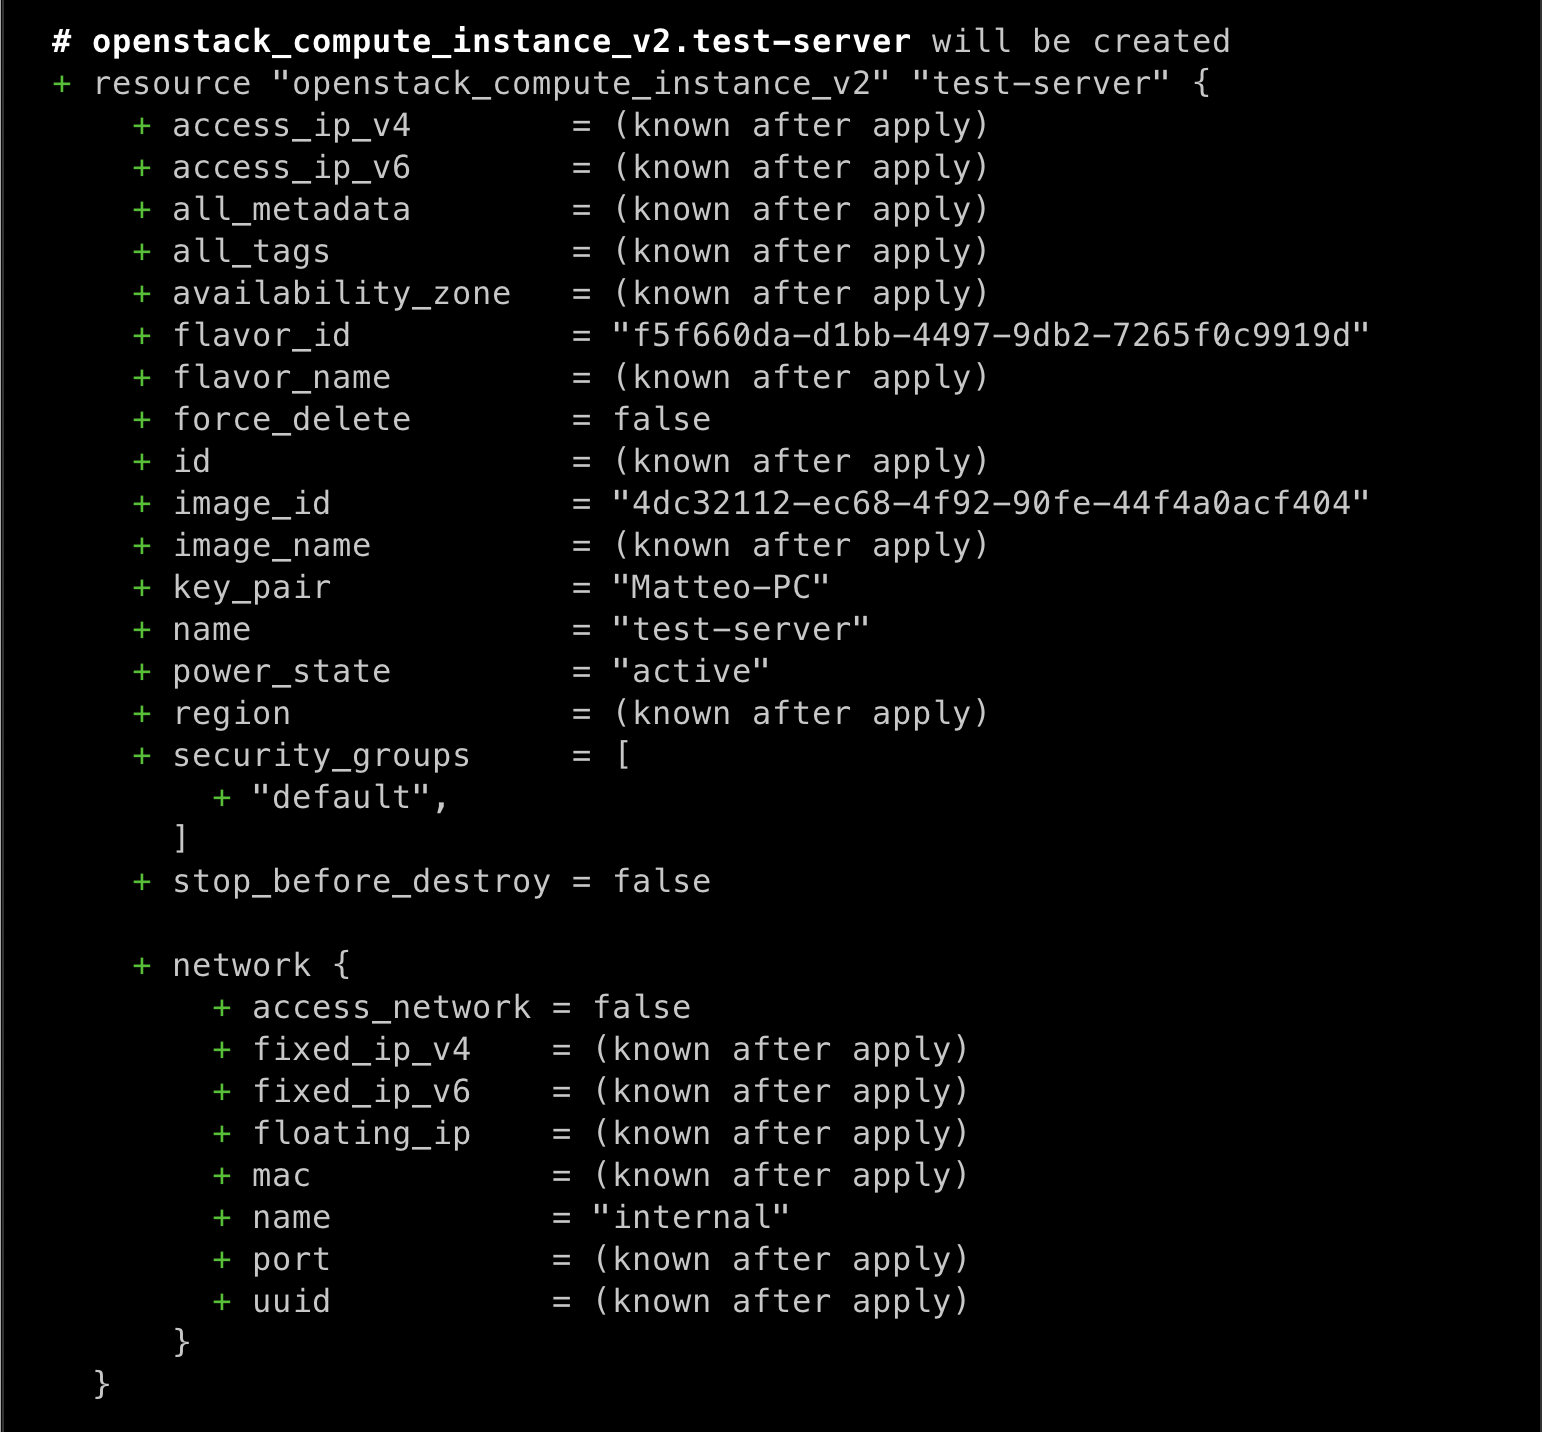
\includegraphics[scale=0.35]{tesi/files/immagini/terraform/projects/project1_terraform_apply.png}
    \caption{Pianificazione delle modifiche all'infrastruttura}
    \label{fig:terraform_project1_apply}
\end{figure}

\subsection{Progetto 2: infrastruttura completa}

Il secondo progetto sviluppato è ovviamente un'evoluzione del primo e prevede la configurazione tramite Terraform di un'infrastruttura completa. Per infrastruttura completa si intende che la configurazione deve includere sia le istanze che tutta la parte di networking.

In questo caso la struttura del progetto rimane abbastanza semplice ma sono stati aggiunti alcuni file in modo mantenere tutto il codice più organizzato. Di seguito è riportato uno schema della struttura del progetto:
\dirtree{%
.1 02\_full\_infrastructure.
.2 example.tfvars.
.2 instances.tf.
.2 main.tf.
.2 networking.tf.
}

In \cref{app:tf_proj2} è possibile vedere tutti i file di questo progetto compresi quelli che non vengono mostrati qui per motivi di spazio.

\paragraph{Variabili di input.} All'interno di questo progetto sono state aggiunte alcune variabili di input. Queste variabili sono dichiarate all'interno del file \verb|main.tf| nel seguente modo:
\lstinputlisting[language=hcl,caption={},firstline=12,lastline=45]{tesi/files/terraform_projects/02_full_infrastructure/main.tf}
\noindent
Come si può notare ciascuna variabile dichiarata è di tipo \code{object} e al suo interno contiene altre variabili di tipi differenti. Quando si esegue il deployment tramite Terraform è necessario specificare un file tramite l'argomento \verb|-varfile| che contiene le assegnazioni dei valori a queste variabili. All'interno del progetto è presente infatti il file \verb|example.tfvars| che contiene appunto un esempio di come deve essere strutturato un file con tutte le variabili di questo progetto assegnate.
\lstinputlisting[language=hcl,caption={}]{tesi/files/terraform_projects/02_full_infrastructure/example.tfvars}
La sintassi generica per poter accedere alle variabili definite all'interno del progetto è la seguente: \code{var.<nome\_variabile>}; dato che le variabili definite qui contengono a loro volta altre variabili per accedere ad esempio al nome dell'utente la sintassi è la seguente: \code{var.auth.user}.

\paragraph{Networking.} Tutte le configurazioni riguardanti la rete dell'infrastruttura si trovano nel file \verb|networking.tf|. Al suo interno ci sono 5 blocchi di tipo \code{resource} utilizzati per configurare le seguenti risorse:
\begin{itemize}
    \item network
    \item subnet
    \item security group da assegnare all'istanza
    \item router
    \item interfaccia che collega il router alla subnet definita in precedenza
\end{itemize}

Nel \cref{lst:project2_router_interface} è riportato il blocco che configura il collegamento del router alla subnet tramite una nuova interfaccia.
\lstinputlisting[language=hcl,label={lst:project2_router_interface},caption={Configurazione dell'interfaccia del router che lo collega alla subnet},firstline=33,lastline=36]{tesi/files/terraform_projects/02_full_infrastructure/networking.tf}
\noindent
Come si può notare gli unici due argomenti sono l'ID del router e l'ID della subnet a cui l'interfaccia si deve collegare. Questo esempio è interessante perché mostra come è possibile utilizzare gli argomenti di determinate risorse per configurarne altre. Nello specifico la sintassi utilizzata per accedere agli argomenti di altre risorse è la seguente: \code{<tipo\_risorsa>.<etichetta\_risorsa>.<parametro>}. Se ad esempio si volesse accedere all'argomento \code{router\_id} dell'interfaccia creata dall'esempio sopra la sintassi sarebbe la seguente: \\
\code{openstack\_networking\_router\_interface\_v2.tf\_router\_interface.router\_id}.

\paragraph{Istanza}

Tutte le configurazioni riguardanti l'istanza si trovano all'interno del file \verb|instances.tf|. Il blocco riguardante l'istanza stessa è molto simile a quello del progetto precedente con una sola eccezione: in questo caso è stato aggiunto un altro blocco al suo interno chiamato \code{block\_device} (riportato nel \cref{lst:project2_block_device}) che permette di collegare un volume all'istanza.
\lstinputlisting[
    language=hcl,
    label={lst:project2_block_device},
    caption={Configurazione di un volume collegato all'istanza},
    firstline=7,
    lastline=14
]{tesi/files/terraform_projects/02_full_infrastructure/instances.tf}

All'interno del file \verb|instances.tf| è anche presente la configurazione del floating IP e l'assegnazione di quest'ultimo all'istanza creata.


\subsection{Progetto 3: Proof of Concept}

Il terzo progetto è l'ultima iterazione e sfrutta tutte le funzionalità offerte dal cloud OpenStack installato. Lo scopo è quello di simulare il deployment di un'applicazione web reale creando più istanze e configurando un load balancer in modo che divida le richieste tra di esse. In \cref{fig:terraform_project3_network_topology} è raffigurata la topologia di rete (escluso il load balancer); come si può vedere sono presenti 3 istanze collegate ad una rete privata alla quale è collegato anche un router che permette alle suddette istanze di accedere a internet. Il load balancer è configurato in modo da essere collegato sia alla rete pubblica che a quella privata così da poter essere raggiungibile dai client e potersi collegare alle istanze tramite la rete interna.

\begin{figure}[H]
    \center
    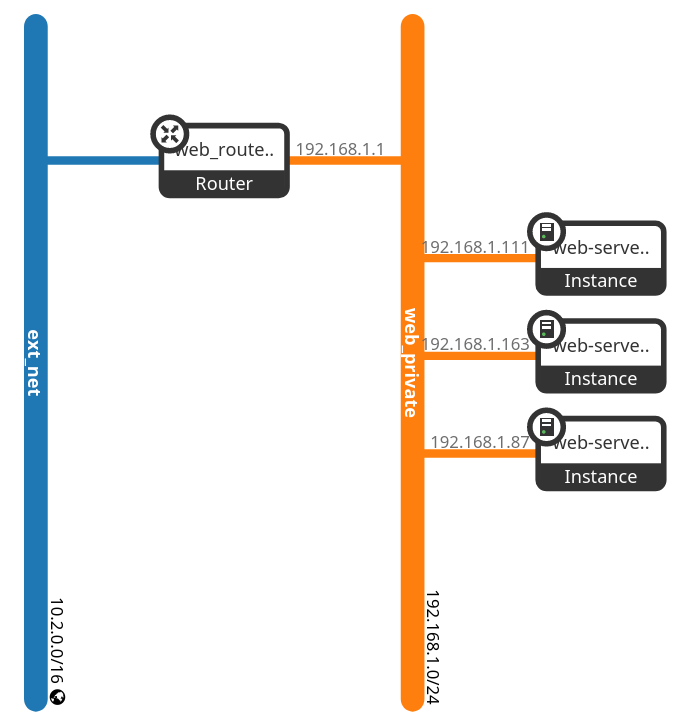
\includegraphics[scale=0.5]{tesi/files/immagini/terraform/projects/project3_network_diagram.png}
    \caption{Topologia di rete del progetto}
    \label{fig:terraform_project3_network_topology}
\end{figure}

Il progetto ha la seguente struttura:
\dirtree{%
.1 03\_proof\_of\_concept.
.2 example.tfvars.
.2 init-instance.sh.
.2 instances.tf.
.2 load\_balancer.tf.
.2 main.tf.
.2 networking.tf.
.2 output.tf.
}
\noindent
Tutti i file del progetto compresi quelli non riportati in questa sezione possono essere consultati in \cref{app:tf_proj3}

\paragraph{Istanze.}

La configurazione delle istanze si trova all'interno del file \\
\verb|instances.tf| che, rispetto al progetto precedente, presente 2 aggiunte: l'argomento \code{count} che permette di specificare il numero di istanze da creare e il parametro \code{user\_data} che permette di specificare uno script bash che sarà poi eseguito dalle macchine all'avvio. La porzione di configurazione dell'argomento \code{user\_data} è la seguente:
\lstinputlisting[language=hcl,caption={},firstline=10,lastline=12]{tesi/files/terraform_projects/03_proof_of_concept/instances.tf}
\noindent
In questo caso viene utilizzata la funzione \code{templatefile} per caricare uno script da file e nello specifico carica il file chiamato \verb|init-instance.sh| contenuto nella directory principale del modulo; il secondo argomento di tale funzione è un oggetto che permette di inoltrare variabili allo script (in questo caso \code{instance\_idx}. Lo script \verb|init-instance.sh| è molto semplice ed è riportato di seguito:
\lstinputlisting[language=mybash,caption={}]{tesi/files/terraform_projects/03_proof_of_concept/init-instance.sh}
\noindent
Il suo compito è quello di installare Apache Web Server e di creare un file \verb|index.html| all'interno del quale viene scritto l'indice della macchina appena creata. In questo modo ciascuna macchina creata avrà un indice diverso e, accedendo attraverso il load balancer, sarà possibile capire a quale macchina ci si sta connettendo e verificare che l'algoritmo di load balancing stia funzionando come ci si aspetta.

\paragraph{Load Balancer.}

Tutte le configurazione del load balancer si trovano all'interno del file \verb|load_balancer.tf|. Di seguito è riportata la configurazione del pool che potrebbe essere interessante perché contiene un blocco dinamico:
\lstinputlisting[language=hcl,caption={},firstline=7,lastline=29]{tesi/files/terraform_projects/03_proof_of_concept/load_balancer.tf}
\noindent
Il primo blocco di questa configurazione è quello che definisce il pool; si può notare come l'algoritmo utilizzato per il load balancing è round robin e che il protocollo specificato per la connessione agli host è HTTP. Il secondo blocco invece è la configurazione dei membri del pool; al suo interno si trova un altro blocco dinamico chiamato \code{"member"} che itera le istanze creando per ciascuna un blocco contenente come argomenti l'indirizzo IP, la porta su cui è esposto il servizio e il peso (utilizzato durante il load balancing per dare priorità di connessione ad una macchine rispetto alle altre).

Sono inoltre configurati un listener sulla porta 80 con protocollo HTTP e un health monitor che esegue periodicamente richieste HTTP alle istanze per verificare che siano ancora online e che il web server stia funzionando correttamente.

\paragraph{Output.}

Terraform permette di definire un output che viene generato una volta completate le modifiche e permette di visualizzare alcune informazioni potenzialmente molto utili sull'infrastruttura appena creata. All'interno del file \verb|output.tf| sono presenti due blocchi di tipo output:
\lstinputlisting[language=hcl,caption={}]{tesi/files/terraform_projects/03_proof_of_concept/outputs.tf}
\noindent
Il primo blocco mostra il floating IP assegnato al load balancer mentre il secondo mostra i dettagli di tutte le istanze create. In \cref{fig:terraform_project3_output} è mostrato un esempio di quello che viene scritto in output dichiarando questi due blocchi.

\begin{figure}[H]
    \center
    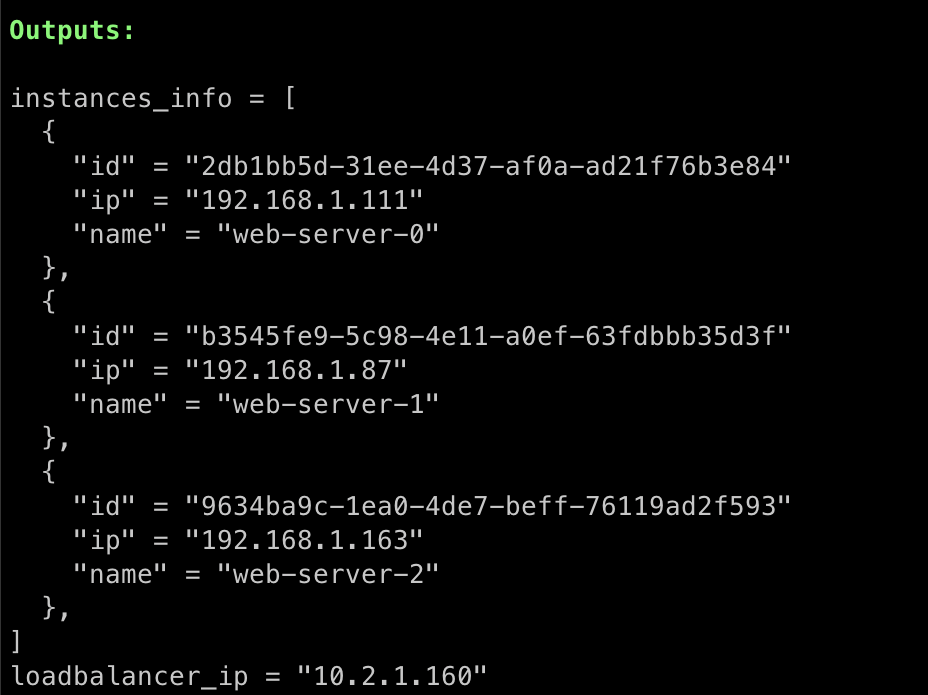
\includegraphics[scale=0.6]{tesi/files/immagini/terraform/projects/project3_output.png}
    \caption{Output di terraform}
    \label{fig:terraform_project3_output}
\end{figure}
